\documentclass[11pt,a4paper]{article}
\usepackage[a4paper,margin=2.5cm]{geometry}
\usepackage{amsmath}
\usepackage{libertinus} % loads unicode-math under XeTeX
\usepackage{graphicx}
\usepackage{booktabs}
\usepackage{float} % [H]: appendix tables stay under their headings
\usepackage{tabularx}
\usepackage{fvextra}
\usepackage{enumitem}
\usepackage[authoryear,round]{natbib}
\usepackage[font=small,labelfont=bf]{caption}
\usepackage{xcolor}
\usepackage{xurl}
\usepackage[hidelinks]{hyperref}
\hypersetup{pdftitle={How much does product classification cost in basis points?},
  pdfauthor={Thanatchon Chongmankhong}}
\usepackage{microtype}

\graphicspath{{../figures/out/}}
% Generated by `cpilens report` from results/. Do not edit by hand.
\newcommand{\InScopeWeightEqual}{40.5}
\newcommand{\InScopeWeightNnls}{43.5}
\newcommand{\LLMSpendUSD}{5.62}
\newcommand{\NCorpusTexts}{88{,}622}
\newcommand{\NGoldDouble}{150}
\newcommand{\NGoldSample}{600}
\newcommand{\NGoldStrata}{13}
\newcommand{\NLLMCalls}{9{,}555}
\newcommand{\NLabelsInScope}{28}
\newcommand{\NMocSpecs}{31{,}822}
\newcommand{\NMocTest}{6{,}017}
\newcommand{\NMocTrainval}{25{,}805}
\newcommand{\NOffMarkets}{18}
\newcommand{\NOffProducts}{76{,}269}
\newcommand{\NOffThailand}{10{,}526}
\newcommand{\NOffThailandSilver}{4{,}415}
\newcommand{\NOffThailandThaiScript}{7{,}303}
\newcommand{\NWeakNonthai}{52{,}255}
\newcommand{\NWeakThai}{3{,}945}

% \input is not expandable inside a tabular; this reads generated table rows
\makeatletter\newcommand{\inputrows}[1]{\@@input #1 }\makeatother

\title{How much does product classification cost in basis points?\\[0.3em]
\large Multilingual classification of Thai product text for consumer price measurement}
\author{Thanatchon Chongmankhong\thanks{The views expressed are the author's own and do not
necessarily reflect those of the Bank of Thailand. This work uses only publicly available data.
Code and derived data: \url{https://github.com/thanatchon36/cpilens}.}}
\date{October 2026}

\begin{document}
\maketitle

\begin{abstract}
Web and scanner prices enter a consumer price index only after each product has been
assigned to an item of the official basket. We ask what that classification step costs in
measured inflation. Using public Thai data only, we score multilingual text embeddings, a
fine-tuned encoder, LLM prompting and cascades on \NRefSpecs{} held-out official
price-collection specifications, weight every score by CPI expenditure, and pass each
method's confusion matrix through a simulator of the Thai CPI. Transfer from non-Thai
products alone classifies \AccWEfiveMLPZeroShot\% of the evaluated weight correctly, and all
official labels raise this to \AccWEfiveMLP\%. A frontier LLM reaches \AccWOpus\%, and a cascade
matches it at \CostPctCasEfiveMLPOpus\% of its cost. With the LLM's confusion matrix, headline
year-on-year inflation would be misstated by \BpYoyRmseHeadlineOpus{} basis points (RMSE);
with an embedding classifier, by \BpYoyRmseHeadlineEfiveMLP. Accuracy does not rank methods by
this error. Code and derived data are open.

\end{abstract}

\noindent\textbf{JEL codes:} C55, C81, E31.\quad % numbers-ok: JEL codes
\textbf{Keywords:} consumer price index, product classification, multilingual text embeddings,
large language models, web prices, measurement error, Thailand.

\section{Introduction}\label{sec:introduction}

Statistical offices and central banks increasingly measure prices from retailers' websites
and scanner data \citep{cavallo2016bpp, eurostat2017scanner, eurostat2020webscraping}. These
sources carry millions of products, but a product enters a consumer price index only after it
has been assigned to an item of the official basket. Done by hand, that step does not scale;
done by a model, it introduces an error. The literature on classification for price
statistics reports this error as accuracy \citep{martindale2020semi, harms2019cbs,
bis2026spectrum}. A central bank does not target accuracy. It needs to know how far measured
inflation would move.

This paper puts that question to one language and one index. We classify Thai product text
into the in-scope items of the Thai CPI with four families of method: multilingual text
embeddings with simple classifiers, a fine-tuned multilingual encoder, few-shot prompting of
two commercial LLMs, and cascades that send a cheap classifier's unsure products to an LLM.
We score them on \NRefSpecs{} held-out official price-collection specifications, published
by the Ministry of Commerce with their official item codes, and weight every score by CPI
expenditure. We then pass each method's confusion matrix through a simulator of the Thai CPI,
built from public weights and item indices, which returns the error the classifier would add
to measured headline, food and core inflation in basis points. Three questions organise the
paper.

\emph{RQ1: how far does transfer from other languages go, and what are official labels
worth?} Thai labelled product data are scarce, while Open Food Facts holds millions of
products in other languages. An \NameEfive{} classifier trained only on non-Thai products
classifies \AccWEfiveMLPZeroShot\% of the evaluated CPI weight correctly. Up to
\CfgBudgetMax{} official labels add little, and all \NMocTrainval{} of them raise it to
\AccWEfiveMLP\%.

\emph{RQ2: what does accuracy cost?} On official Thai text the LLMs are far ahead:
\NameOpus{} reaches \AccWOpus\% and \NameHaiku{} \AccWHaiku\%, against \AccWXlmrFT\% for the
best cheap method. A cascade from the \NameEfive{} classifier to \NameOpus{} matches
\NameOpus{} at \CostPctCasEfiveMLPOpus\% of its cost. Most of the remaining LLM error comes from
two places where our description of the items differed from the office's practice, not from
misreading Thai.

\emph{RQ3: what does classification error cost in basis points?} With \NameOpus's confusion
matrix, headline year-on-year inflation would be misstated by \BpYoyRmseHeadlineOpus{} basis
points (RMSE; \CfgCI\% interval \BpYoyRmseHeadlineOpusLo--\BpYoyRmseHeadlineOpusHi) and food
inflation by \BpYoyRmseFoodOpus. With the \NameEfive{} classifier the errors are
\BpYoyRmseHeadlineEfiveMLP{} and \BpYoyRmseFoodEfiveMLP{} basis points. Accuracy does not rank
methods by this error: two classifiers with the same weighted accuracy differ several-fold in
basis points, because what matters is whether the confused items' prices moved apart.

The paper makes three contributions. First, it turns a confusion matrix into basis points of
measured inflation, with a decomposition that attributes the error to individual confusions
and an uncertainty band that reflects how few observations some rows rest on. The simulator
needs only public weights and item indices, so any office can apply it to its own
classifier. Second, it evaluates classification for a CPI in a non-European language, on
the office's own held-out specifications and with expenditure weights on both accuracy and
coverage. Third, the whole pipeline is public and reproducible: it uses only open data, every
number in the paper is generated by code, and the LLM runs cost USD \LLMSpendUSD{} in total.

The closest work is the BIS Innovation Hub's Project Spectrum \citep{bis2026spectrum}, which
classifies euro-area web prices and names testing other languages and back-testing indices as
next steps \citep[p.~30]{bis2026spectrum}. Our taxonomy, language, product universe and
labels differ from Spectrum's, so our numbers are not directly comparable with theirs.
Section~\ref{sec:related} reviews the literature, Section~\ref{sec:data} describes the data
and Section~\ref{sec:methods} the methods. Section~\ref{sec:results} answers the three
questions, Section~\ref{sec:discussion} draws lessons for central banks in Asia,
Section~\ref{sec:limitations} lists the limitations and Section~\ref{sec:conclusion}
concludes.

\section{Related work}\label{sec:related}

% Written after the gold evaluation, from results only.
\textit{[This part is written once the gold labels are evaluated.]}

\section{Data}\label{sec:data}

All data are public. Table~\ref{tab:sources} in Appendix~\ref{app:repro} lists the sources
and their licences; the repository records the retrieval date and checksum of every file.

\subsection{The Thai CPI}

The Thai consumer price index is compiled monthly by the Trade Policy and Strategy Office
(TPSO) of the Ministry of Commerce. The current base year is 2566 in the Buddhist era (2023),
and the series on this base has been in use since January 2568 (2025)
\citep{tpso2025cpinote}. Like most national CPIs it is a Lowe index
\citep{imf2020cpimanual}: expenditure weights from a base period, price-updated to a price
reference month, here December 2567. TPSO's open API publishes monthly indices for the
headline, divisions, groups and items \citep{tpso2026api}. It publishes no weights. The
monthly release publishes price-updated weight shares for the official aggregates only
(headline, the divisions, the food groups and the analytical series such as core CPI). We
recover those shares from the releases and check that they add up the hierarchy and
reproduce the official headline from the published sub-indices.

Below the published aggregates, item weights are not public. We partition the item codes
into \emph{cells}: each official aggregate owns the items whose deepest published ancestor it
is, and the cell weight is the aggregate's weight minus that of the published aggregates
nested below it. Within a cell we estimate item weights in two ways and report both: an equal
split (primary) and non-negative least squares on the Lowe identity, which chooses the split
that best reproduces the cell's index from its items' indices (sensitivity). Neither is an
official weight, and the paper never calls it one.

\subsection{Scope: the items a product classifier can reach}

A classifier of packaged-product text can only measure items sold as packaged products. We
define \NLabelsInScope{} in-scope CPI items: food at home, ready-to-eat food, non-alcoholic
beverages, alcoholic beverages, tobacco, personal care and cleaning products. Each is mapped
to its COICOP 2018 class \citep{unsd2018coicop}. Everything else (rents, energy, transport,
services, clothing, durable goods) is out of scope (\textsc{oos}). In-scope items carry
\InScopeWeightEqual\% of the headline weight under the equal split and \InScopeWeightNnls\%
under NNLS, most of it food (Figure~\ref{fig:coverage}).

\begin{figure}[t]
\centering
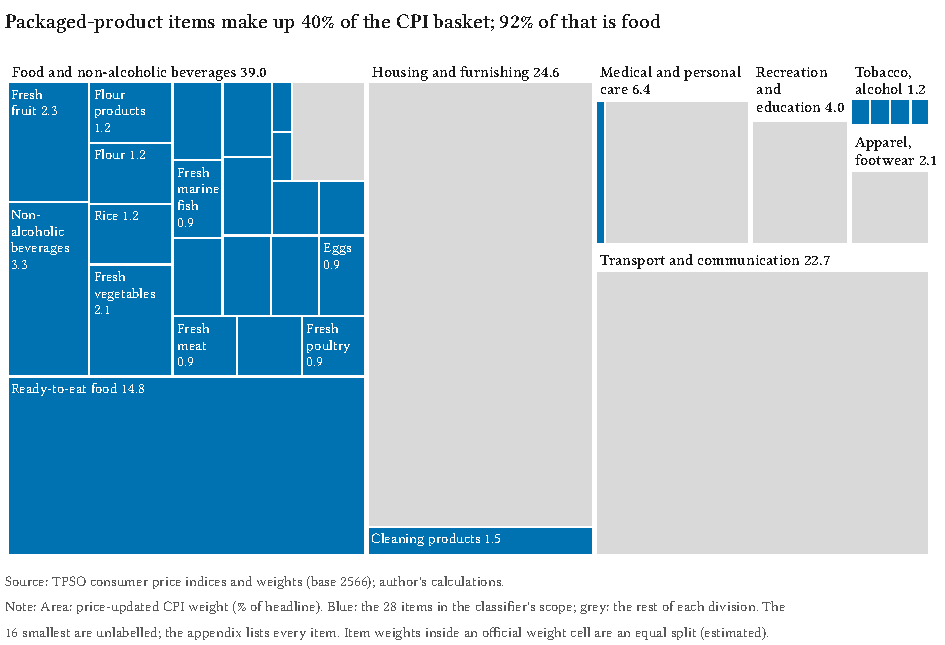
\includegraphics[width=\textwidth]{fig02_coverage.pdf}
\caption{\textbf{Packaged-product items are a large share of the Thai CPI basket, and most of
it is food.} Area: price-updated CPI weight (\% of headline), by division; blue, the
in-scope items; grey, the rest of each division. Item weights inside an official weight cell
are an equal split (estimated). Source: TPSO; author's calculations.}
\label{fig:coverage}
\end{figure}

\subsection{Product text}

\paragraph{Open Food Facts.} Open Food Facts (OFF) is a crowd-sourced, openly licensed
database of packaged products \citep{off2026}. We use its Parquet export and that of its
sister project Open Beauty Facts. Our extract holds \NOffProducts{} products from
\NOffMarkets{} markets: Thailand, other Asian markets and a sample of European products.
Of the \NOffThailand{} products tagged as sold in Thailand, \NOffThailandThaiScript{} have a
name in Thai script. Model input is the product's name, brand and quantity, joined as
\texttt{name | brand | quantity}.

\paragraph{Weak labels.} OFF products carry crowd-sourced category tags. A hand-curated
crosswalk maps tags to CPI items, following TPSO's own item headings rather than intuition
about COICOP (for example, snacks belong to flour products in the Thai CPI). This gives weak
labels: \NWeakNonthai{} non-Thai products and \NWeakThai{} Thai products. Weak labels are
used for training and development, never for evaluation.

\paragraph{Official specifications.} The Ministry of Commerce publishes the product
specifications TPSO uses for price collection: short Thai descriptions with brand and pack
size, each under an official item code \citep{moc2026specs}. These give \NMocSpecs{}
official labels. They are not shop listings, but they are the closest public analogue of
labelled Thai product text. We split them by item code, so that specifications of one item
never straddle training and test: \NMocTrainval{} for training and validation, \NMocTest{}
for test.

\subsection{Gold labels}\label{sec:gold}

Evaluation uses a gold sample of Thai OFF products labelled by the author. The frame is the
\NOffThailandThaiScript{} Thai-market products with a Thai-script name. The sample of
\NGoldSample{} products is stratified by the CPI weight cell of the product's weak label
(\NGoldStrata{} strata, including products with no weak label), with a floor per stratum and
the rest allocated half by stratum size and half by cell weight, so heavily weighted items
are well represented. Inclusion probabilities are stored and every gold estimate is design
weighted. Gold products, and any training text identical to a gold text, are removed from
every training pool.

The labelling tool shows the product's names, brand, quantity and front image, and a search
over the Thai and English item names. It never shows a model's prediction, the weak label or
the stratum. Besides the items and \textsc{oos}, the labeller can answer ``cannot tell from
the information shown'' (\textsc{unk}, excluded from accuracy and counted) and flag any label
as unsure. A random \NGoldDouble{} of the sample is labelled a second time, blind, in a
different order and at least \CfgGapHours{} hours after the first label. Because both passes
are by the same person, their disagreement measures intra-annotator consistency, a lower
bound on the disagreement between two annotators.

\section{Methods}\label{sec:methods}

Figure~\ref{fig:pipeline} summarises the pipeline. Every method maps a product text to one
of the \NLabelsInScope{} in-scope items or \textsc{oos}, with a calibrated confidence; some
may abstain.

\begin{figure}[t]
\centering
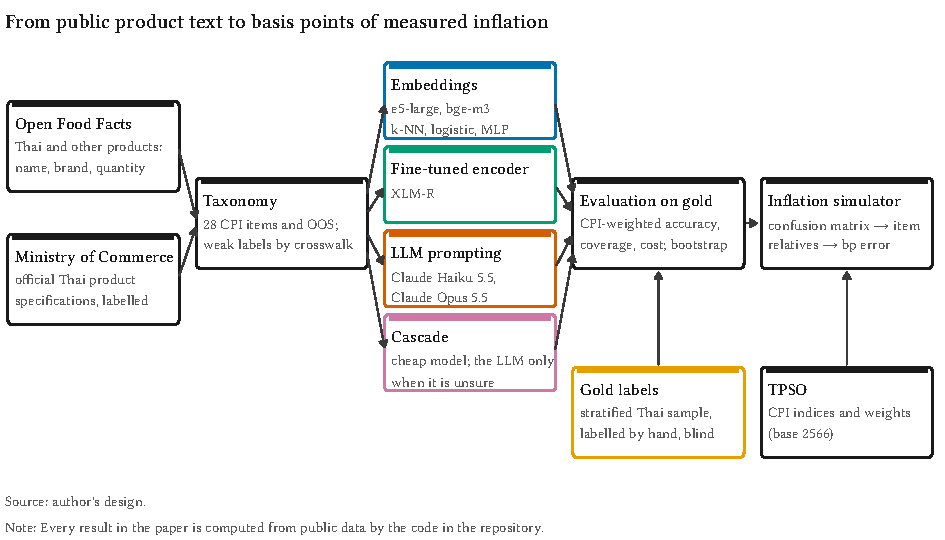
\includegraphics[width=\textwidth]{fig01_pipeline.pdf}
\caption{\textbf{The pipeline runs from public product text to basis points of measured
inflation.} Data sources (left) feed a taxonomy and weak labels, four families of classifier,
an evaluation on hand-labelled gold data and the inflation simulator. Source: author's
design.}
\label{fig:pipeline}
\end{figure}

\subsection{Classifiers}

\paragraph{Frozen multilingual embeddings.} Following Spectrum's design \citep[pp.~3, 19--20]{bis2026spectrum}, the
first family embeds each text once and trains a light classifier on the vectors.
We use two open multilingual embedding models run locally, \NameEfive{}
\citep[\texttt{\HfEfive};][]{wang2024me5} and \NameBge{} \citep[\texttt{\HfBge};][]{chen2024bgem3}.
On top of each we fit three classifiers: cosine $k$-nearest neighbours with
similarity-weighted votes, $k \in \{\CfgKs\}$ chosen on validation macro recall; multinomial
logistic regression; and a one-hidden-layer perceptron (\CfgMLPHidden{} units, dropout
\CfgDropout). The last two share one trainer: Adam with learning rate \CfgLR{} and weight
decay \CfgWeightDecay, class weights proportional to the inverse square root of class
frequency, and early stopping on validation loss (patience \CfgPatience).

\paragraph{Fine-tuned encoder.} XLM-R base \citep[\texttt{\HfXlmr};][]{conneau2020xlmr} with a
classification head, fine-tuned end to end on the same training pools with the same class
weights and early stopping (\CfgFtEpochs{} epochs at most, batch \CfgFtBatch, AdamW at
\CfgFtLR{} with linear warm-up and decay, inputs truncated to \CfgFtMaxLen{} tokens).

\paragraph{LLM prompting.} Two models of different cost, \NameOpus{} and \NameHaiku{}, through
the Anthropic API, one product per request. A fixed system prompt gives the instructions, the
item list grouped by CPI group with short descriptions grounded in TPSO's item headings, and
\CfgFewShot{} official specifications per item drawn from the training split
(Appendix~\ref{app:prompt}). The answer is constrained by a JSON schema: the model names the
group, then an item inside it, and a verbalised confidence, the probability in per cent that the item is right. Refusals count as
abstentions. Every response is cached and every billed call is logged with its tokens and
cost; total spend was capped at USD~\CfgCapUSD{} and came to USD~\LLMSpendUSD.

\paragraph{Cascade.} A cheap classifier answers when its calibrated confidence is at least a
threshold $t$; otherwise the product is routed to an LLM. We pair the cheap classifiers with
each LLM. For each pair, $t$ is the threshold with the highest weighted accuracy on the Thai
weak-label validation split, with ties broken by lower cost. It is fixed before the
reference set is touched, which then scores that one threshold.

\paragraph{Training data and the learning curve (RQ1).} Each embedding classifier is trained
on a sequence of pools: non-Thai weak labels only (zero-shot cross-lingual transfer to Thai);
plus Thai weak labels; plus $n \in \{\CfgBudgets\}$ or all official Thai labels; and official
labels alone. The budget $n$ counts every official label a run touches, validation included,
so a small-budget run cannot tune on thousands of extra official labels.

\paragraph{Calibration.} Each run's logits are divided by one scalar temperature fitted on its
own validation rows by negative log-likelihood \citep{guo2017calibration}; for $k$-NN the
logits are log vote shares. The calibrated top-class probability is the confidence used by
the coverage frontier and the cascade.

\subsection{Evaluation}

\paragraph{Expenditure-weighted accuracy.} What matters for a price index is not how many
products are classified correctly but how much CPI weight is measured correctly. Let $w_k$ be
the CPI weight of item $k$ and $r_k$ the recall of item $k$ on the reference set, estimated
with the design weights $1/\pi_i$ of Section~\ref{sec:ref} \citep{horvitz1952}. The headline
metric is
\begin{equation}
\mathrm{acc}_w = \frac{\sum_k w_k\, r_k}{\sum_k w_k}, \qquad
r_k = \frac{\sum_{i:\, y_i = k} \mathbb{1}[\hat y_i = k]/\pi_i}{\sum_{i:\, y_i = k} 1/\pi_i},
\label{eq:accw}
\end{equation}
the CPI-weighted mean recall over the evaluated items, a weighted version of Spectrum's
in-class recall \citep[p.~22]{bis2026spectrum}. We also report accuracy over the whole
held-out list, which counts \textsc{oos} specifications, and macro-F1. Abstentions are
errors at full coverage.

\paragraph{Coverage, cost and uncertainty.} Sweeping a confidence threshold traces a
weighted accuracy--coverage frontier \citep{geifman2017selective}: the CPI-weighted share of
products answered against $\mathrm{acc}_w$ on those. Cost per million products is the measured
mean API cost per call plus local compute at an assumed USD~\CfgGpuUSDHour{} per GPU-hour times
measured seconds per item. All intervals come from \CfgBoot{} bootstrap resamples of the
reference set, stratified by item \citep{efron1993bootstrap}. Method comparisons are
paired: every method is scored on the same resamples, and the comparisons were fixed in
code before the reference set was scored.

\subsection{From confusion matrices to basis points (RQ3)}\label{sec:sim}

\paragraph{Setting.} For an aggregate $A$ with member items $i$, the Lowe index satisfies
\begin{equation}
\frac{I_{A,t}}{I_{A,L}} = \sum_{i \in A} \frac{w_i}{W_A}\, R_{i,t}, \qquad
R_{i,t} = \frac{I_{i,t}}{I_{i,L}},
\label{eq:lowe}
\end{equation}
where $L$ is the price reference month, $w_i$ are price-updated weights and
$W_A = \sum_{i\in A} w_i$. We take the official item relatives $R_{i,t}$ as the true price
movement of every product in item $i$. This isolates the error due to classification: a
real web-price index would add sampling, matching and quality-adjustment error on top.

\paragraph{Misclassification.} Let $n_k$ be the universe share of products whose true item is
$k$ and $P$ a method's confusion matrix, $P_{kj}$ the probability that a product of item $k$
is classified as $j$. Item $j$ is then measured from a mixture of the products sent to it:
\begin{equation}
\tilde R_{j,t} = \sum_k \phi_{kj}\, R_{k,t}, \qquad
\phi_{kj} = \frac{n_k P_{kj}}{\sum_{k'} n_{k'} P_{k'j}}.
\label{eq:mix}
\end{equation}
Products sent to \textsc{oos} or abstained on are dropped. If nothing flows into an item, its
weight is redistributed within its CPI group; true \textsc{oos} products that leak into an
item move with the official non-food index. Out-of-scope items are measured perfectly. The
measured index is
\begin{equation}
\hat I_{A,t} = I_{A,t} + I_{A,L} \sum_{j \in A} \frac{w_j}{W_A}
\bigl(\tilde R_{j,t} - R_{j,t}\bigr),
\label{eq:measured}
\end{equation}
and the error is reported in basis points of month-on-month and year-on-year inflation for
the headline, food and core indices. A perfect classifier gives $\tilde R = R$ and reproduces
every official series exactly, which is a unit test of the code.

\paragraph{Product universe.} The shares $n_k$ are not observed: the reference set is the
office's list, not a stream of products. We state them as an assumption and report two
universes. In the primary one, products arrive in proportion to CPI expenditure weights,
with the weight outside the evaluated items arriving as out-of-scope products; in the
alternative they arrive in proportion to the office's specification list, that is, the
design-weighted shares of the reference set. In-scope items without specifications are held
at their official values, like out-of-scope items.

\paragraph{Decomposition.} Since $\sum_k \phi_{kj} = 1$,
$\tilde R_{j,t} - R_{j,t} = \sum_k \phi_{kj}(R_{k,t} - R_{j,t})$. The contribution of each
confusion $k \to j$ is therefore the item weight times the misallocated mass times the gap
between the two items' price movements. A confusion matters only if it is frequent, falls on
a heavily weighted item and joins items whose prices move differently.

\paragraph{Uncertainty.} The confusion counts come from the reference set. We draw
\CfgDraws{} confusion matrices from a
Dirichlet posterior, row by row. Sparse rows need a prior, and a flat one is not neutral: it
sends mass to arbitrary items and creates error even for a perfect classifier. We therefore
use an empirical-Bayes prior worth $\alpha = \CfgAlpha$ product per row, whose mean puts the
method's pooled accuracy on the diagonal and spreads the rest over the columns where that
method's errors actually go. Under this prior a perfect classifier has zero error in every
draw. Two variants bracket the result: a perfect classifier on the same universe (any error
left is due to coverage alone) and the method's matrix plus product-level sampling noise,
in which each product's log price drifts from its item's as a random walk with an assumed
annual standard deviation of \CfgSigmaLo\% or \CfgSigmaHi\%, and item $j$ averages the products
sent to it, the size of the held-out list standing in for the number of products.

\section{Results}\label{sec:results}

All scores in this section are on the reference set (Section~\ref{sec:ref}): \NRefSpecs{}
held-out official specifications, \NRefInScope{} of them in scope. Weighted accuracy is
$\mathrm{acc}_w$ of equation~\eqref{eq:accw} under the equal split; brackets give
\CfgCI\% intervals from \NBoot{} stratified bootstrap resamples. The NNLS split is reported
where it changes a conclusion.

\subsection{RQ1: cross-lingual transfer and the value of official labels}\label{sec:rq1}

\textbf{Answer.} Transfer from non-Thai products does most of the work. An \NameEfive{} MLP
trained only on non-Thai products classifies \AccWEfiveMLPZeroShot\%
[\AccWEfiveMLPZeroShotLo, \AccWEfiveMLPZeroShotHi] of the evaluated CPI weight correctly.
Thai weak labels add nothing, budgets of up to \CfgBudgetMax{} official labels add little,
and all \NMocTrainval{} official labels raise it to \AccWEfiveMLP\%
[\AccWEfiveMLPLo, \AccWEfiveMLPHi].

Figure~\ref{fig:learning} traces the learning curve. With Thai weak labels added the score is
\AccWEfiveMLPThaiWeak\%; with \CfgBudgetMax{} official labels on top of the weak ones it is
\AccWEfiveMLPPlusThousand\%. Only the full official set moves it clearly: the paired gain of
all official labels over zero-shot transfer is \DiffEfiveMLPEfiveMLPZeroShot{} percentage
points [\DiffEfiveMLPEfiveMLPZeroShotLo, \DiffEfiveMLPEfiveMLPZeroShotHi]. That gain depends on
how the weight is spread inside the official cells: under the NNLS split it is
\DiffEfiveMLPEfiveMLPZeroShotNnls{} points [\DiffEfiveMLPEfiveMLPZeroShotNnlsLo,
\DiffEfiveMLPEfiveMLPZeroShotNnlsHi], and the interval includes zero. Official labels on their
own need the whole set: with \CfgBudgetMax{} of them the classifier reaches only
\AccWEfiveMLPMocThousand\%, and with all of them \AccWEfiveMLPMocOnly\%. The
other encoders tell the same story at lower levels: zero-shot \NameBge{} MLP reaches
\AccWBgeMLPZeroShot\% and the zero-shot fine-tuned XLM-R \AccWXlmrFTZeroShot\%; with every
label the three are within a few points of one another (\AccWEfiveMLP\%, \AccWBgeMLP\% and
\AccWXlmrFT\%).

\begin{figure}[t]
\centering
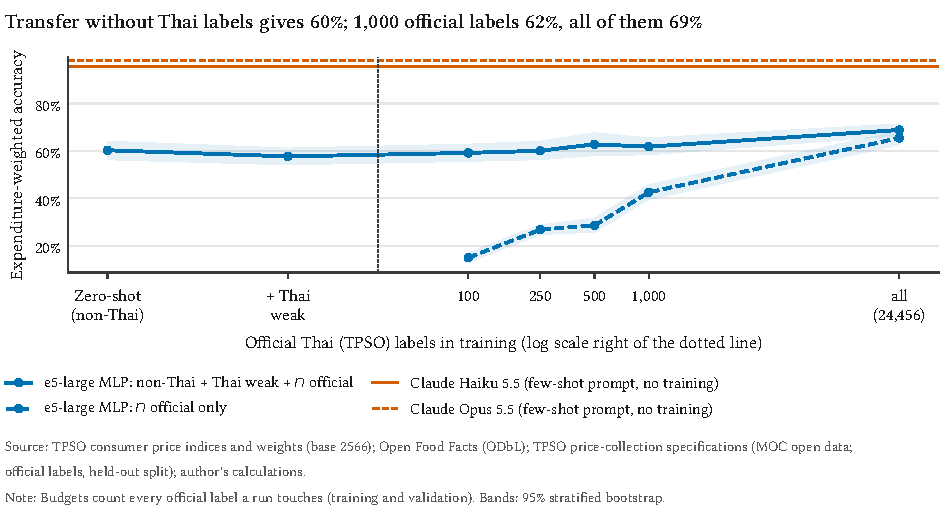
\includegraphics[width=\textwidth]{fig05_learning_curve.pdf}
\caption{\textbf{Transfer from non-Thai products gives \AccWEfiveMLPZeroShot\% weighted
accuracy with no Thai label; \CfgBudgetMax{} official labels give \AccWEfiveMLPPlusThousand\%
and all of them \AccWEfiveMLP\%.} \NameEfive{} MLP by training pool: zero-shot (non-Thai weak
labels), plus Thai weak labels, plus $n$ official labels (solid), and $n$ official labels
alone (dashed). Horizontal lines: the two LLMs, prompted with \CfgFewShot{} official examples
per item. Bands: \CfgCI\% stratified bootstrap. Source: Open Food Facts; MOC; TPSO; author's
calculations.}
\label{fig:learning}
\end{figure}

Plain accuracy hides all of this. The held-out list is mostly out-of-scope
specifications, and a classifier that answers \textsc{oos} to almost everything scores well
on it: the \NameEfive{} MLP trained on a hundred official labels alone is right on
\AccEfiveMLPMocHundred\% of the list but on only \AccWEfiveMLPMocHundred\% of the evaluated
CPI weight. Conversely, the zero-shot classifier is right on only \AccEfiveMLPZeroShot\% of
the list because it was never shown an out-of-scope Thai text, yet it measures most of the
weight correctly. A metric weighted by expenditure is not a refinement here; it reverses the
ranking.

The input fields matter less than the labels. Dropping the brand from the input costs
\DiffEfiveMLPEfiveMLPNoBrand{} points [\DiffEfiveMLPEfiveMLPNoBrandLo,
\DiffEfiveMLPEfiveMLPNoBrandHi]; dropping the quantity costs nothing measurable
(\DiffEfiveMLPEfiveMLPNoQty{} [\DiffEfiveMLPEfiveMLPNoQtyLo, \DiffEfiveMLPEfiveMLPNoQtyHi]).
Figure~\ref{fig:alignment} shows why transfer works for some items and not for others: in
the embedding space, Thai beverages, eggs and dairy products sit among non-Thai products of
the same item, while Thai processed seafood, processed meat and fresh fruit do not.

\begin{figure}[t]
\centering
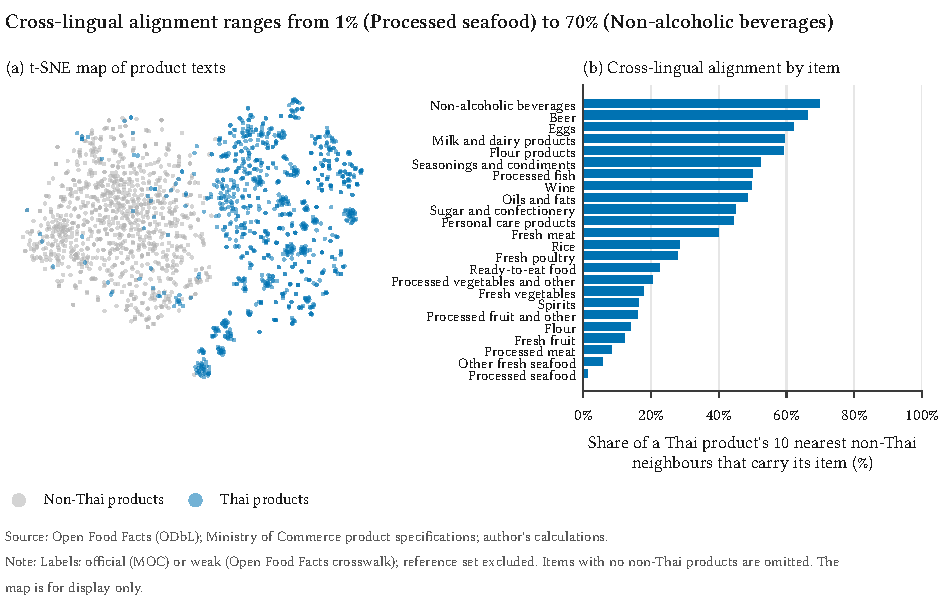
\includegraphics[width=\textwidth]{fig08_embedding_map.pdf}
\caption{\textbf{Thai products sit next to non-Thai products of the same item for some items
and not for others.} (a) t-SNE map of a balanced sample of product texts (display only).
(b) Cross-lingual alignment: the share of a Thai product's \CfgAlignK{} nearest non-Thai
neighbours, in the full \NameEfive{} space, that carry its item. The reference set is
excluded. Source: Open Food Facts; MOC; author's calculations.}
\label{fig:alignment}
\end{figure}

\subsection{RQ2: accuracy, coverage and cost}\label{sec:rq2}

\textbf{Answer.} On official Thai text the LLMs are far ahead.
\NameOpus{} classifies \AccWOpus\% [\AccWOpusLo, \AccWOpusHi] of the evaluated weight correctly
and \NameHaiku{} \AccWHaiku\% [\AccWHaikuLo, \AccWHaikuHi], against \AccWXlmrFT\% for the best
cheap method. A cascade that sends the \NameEfive{} MLP's unsure products to \NameOpus{}
matches \NameOpus{} at \CostPctCasEfiveMLPOpus\% of its cost.

The gap between the LLMs and every cheap method is large and certain: \NameHaiku{} is ahead
of the \NameEfive{} MLP by \DiffHaikuEfiveMLP{} points [\DiffHaikuEfiveMLPLo,
\DiffHaikuEfiveMLPHi], of \NameBge{} by \DiffHaikuBgeMLP{} and of the fine-tuned XLM-R by
\DiffHaikuXlmrFT. \NameOpus{} is ahead of \NameHaiku{} by \DiffOpusHaiku{} points
[\DiffOpusHaikuLo, \DiffOpusHaikuHi] and costs \CostRatioOpusHaiku{} times as much: USD
\CostOpus{} per million products against USD \CostHaiku{}, while the embedding classifiers
cost well under a dollar (USD \CostEfiveMLP{} for the \NameEfive{} MLP;
Figure~\ref{fig:cost}). Under the NNLS split every score falls, because NNLS moves weight
onto the item with the largest LLM error (below), but the ranking does not change
(\NameOpus{} \AccWOpusNnls\%, \NameHaiku{} \AccWHaikuNnls\%, \NameEfive{} MLP
\AccWEfiveMLPNnls\%).

\begin{figure}[t]
\centering
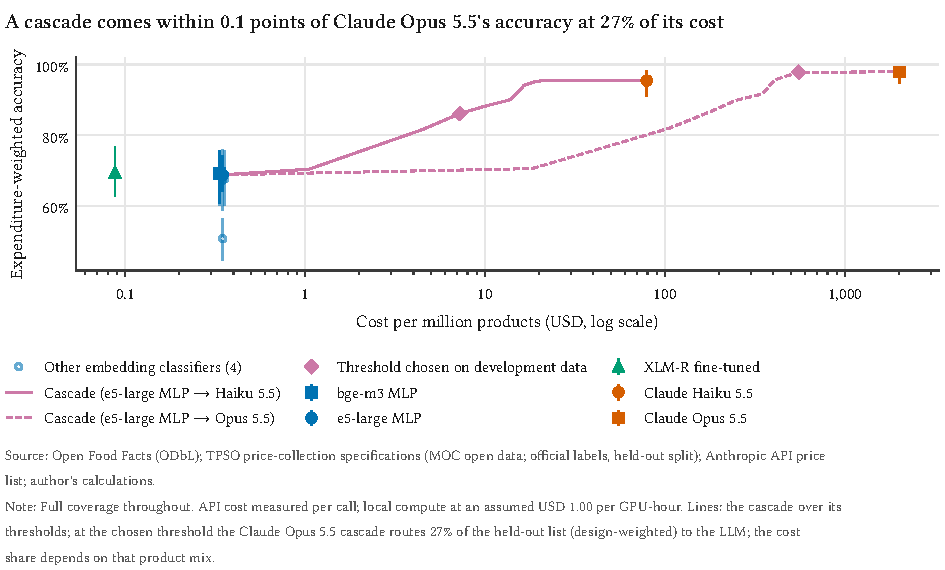
\includegraphics[width=\textwidth]{fig04_cost.pdf}
\caption{\textbf{A cascade from the \NameEfive{} MLP to \NameOpus{} matches \NameOpus{} at
\CostPctCasEfiveMLPOpus\% of its cost; no cheap method comes close to either LLM.} Weighted
accuracy at full coverage against cost per million products (log scale). Lines: each cascade
over its candidate thresholds; diamonds: the threshold chosen on development data. API cost
measured per call; local compute at an assumed USD~\CfgGpuUSDHour{} per GPU-hour. Source:
Open Food Facts; MOC; TPSO; Anthropic API price list; author's calculations.}
\label{fig:cost}
\end{figure}

Cascades work when the threshold is set where the cheap model is reliable. For the
\NameEfive{} MLP and \NameOpus, the development data chose a confidence threshold of
\ThresholdCasEfiveMLPOpus; \RoutedCasEfiveMLPOpus\% of the reference products went to the LLM,
and the cascade scored \AccWCasEfiveMLPOpus\%, a paired difference from \NameOpus{} of
\DiffCasEfiveMLPOpusOpus{} points [\DiffCasEfiveMLPOpusOpusLo, \DiffCasEfiveMLPOpusOpusHi]. The
other cascades were given lower thresholds by the development data (the Thai weak-label
validation split, which is Open Food Facts text), routed fewer products and differed from the
LLM they call by between \DiffCasXlmrFTHaikuHaiku{} and \DiffCasEfiveMLPHaikuHaiku{} points.
Confidence calibrated on one kind of text was too high on the other: a cheap classifier is
confidently wrong on sub-items it has never seen.

Abstaining does not close the gap. Figure~\ref{fig:frontier} trades coverage for accuracy:
the cheap methods gain accuracy as they leave their least confident products unclassified,
but even on the small share of weight they are surest about they stay below the LLMs'
accuracy at full coverage.

\begin{figure}[t]
\centering
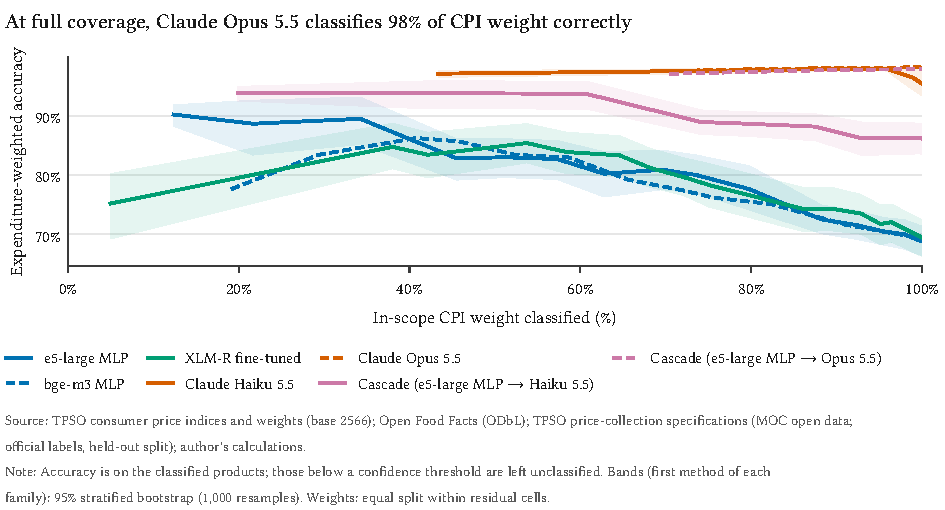
\includegraphics[width=\textwidth]{fig03_frontier.pdf}
\caption{\textbf{At full coverage \NameOpus{} classifies \AccWOpus\% of the evaluated CPI
weight correctly; the cheap methods stay below the LLMs at any coverage.} Weighted accuracy
on the classified products against the in-scope CPI weight classified, as the confidence
threshold rises. Bands (first method of each family): \CfgCI\% stratified bootstrap. Source:
Open Food Facts; MOC; TPSO; author's calculations.}
\label{fig:frontier}
\end{figure}

\paragraph{Where the errors are.} The cheap methods miss whole items. The fine-tuned XLM-R
misses every held-out specification of fresh meat, freshwater fish, processed fish and tobacco
(each a small cell), sends most personal-care specifications to \textsc{oos}, and confuses
seasonings with beverages and cleaning with personal-care products (Figures~\ref{fig:recall}
and~\ref{fig:confusion}); its \NErrXlmrFT{} in-scope errors fall on \NErrSubitemsXlmrFT{}
sub-items. The LLMs' errors are concentrated. \NameOpus's \NErrOpus{} in-scope errors fall on
\NErrSubitemsOpus{} sub-items, and \NErrTopThreeOpus{} of them (\PctErrTopThreeOpus\%) on three;
\NameHaiku's largest three are the same. The TPSO item whose Thai name means ``personal
items'' covers wristwatches, school bags and hair dryers as well as soap and toothpaste. Our
label description, written from the item headings, named only personal-care goods, and both
LLMs sent the held-out wristwatches, school bags and hair dryers to \textsc{oos}. The next
largest error is margarine, which TPSO counts under milk and dairy products and our
description listed under oils and fats; the LLMs followed the description. These are not
failures to read Thai. They are gaps in our documentation of the official item contents, and
they would be closed by better documentation, not by a better model. We did not change the
descriptions after seeing them, since that would tune on the reference set. Because NNLS gives
the personal-items cell a much larger weight than the equal split does, it is this one gap
that lowers the LLM scores under NNLS.

\begin{figure}[t]
\centering
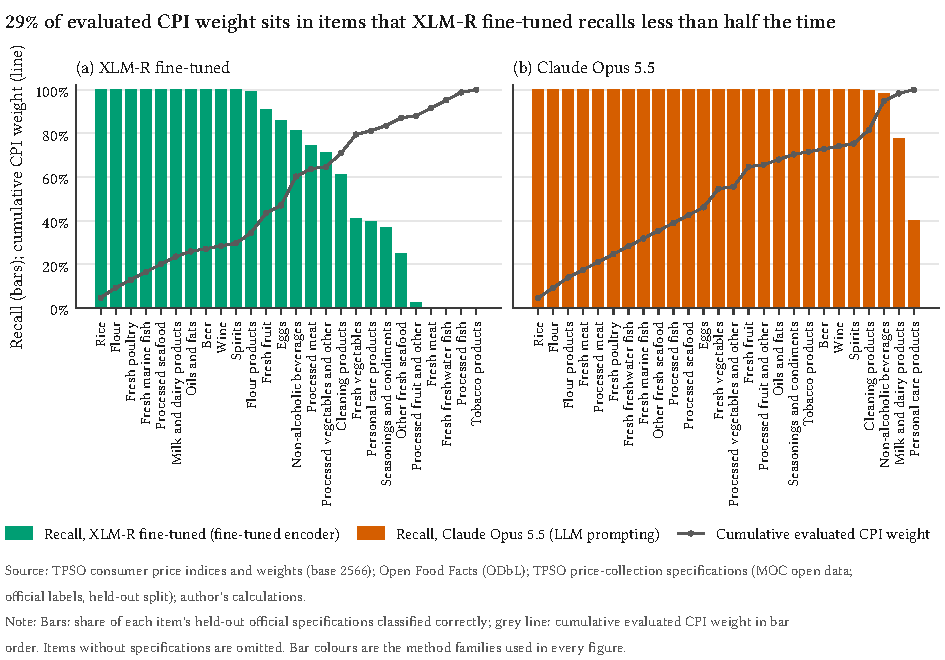
\includegraphics[width=\textwidth]{fig06_item_recall.pdf}
\caption{\textbf{The fine-tuned XLM-R misses whole items; \NameOpus{} misses large parts of
only two.} Recall of each item on the reference set, ranked, with the cumulative in-scope CPI
weight in bar order (line). Items without specifications are omitted. Source: MOC; TPSO;
author's calculations.}
\label{fig:recall}
\end{figure}

\begin{figure}[t]
\centering
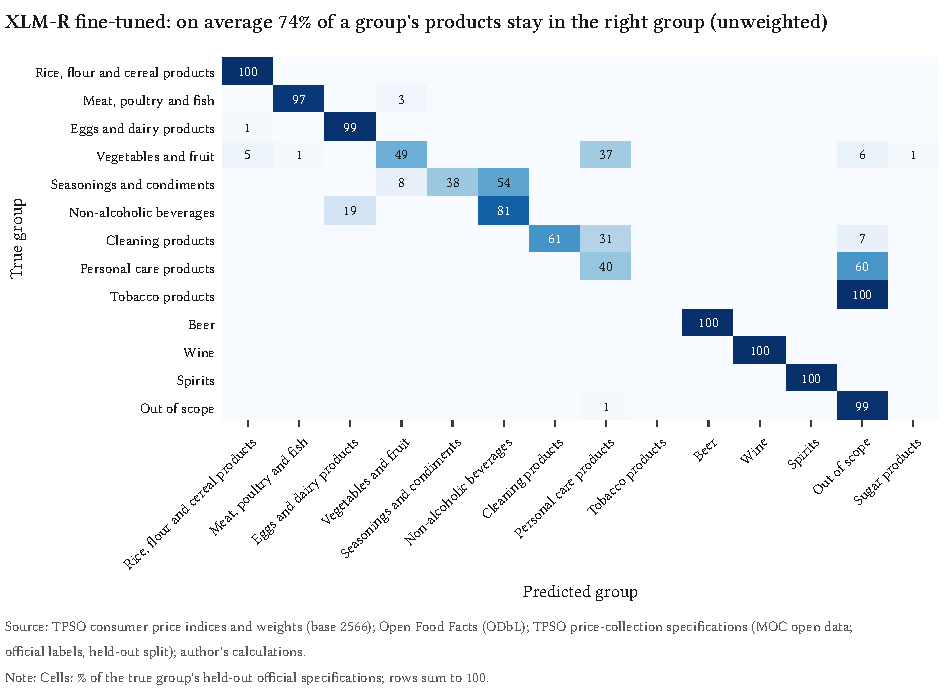
\includegraphics[width=\textwidth]{fig07_group_confusion.pdf}
\caption{\textbf{The best cheap method keeps rice and alcoholic drinks in the right group but
sends tobacco and most personal-care products out of scope and mixes seasonings with beverages
and cleaning with personal-care products.}
Row-normalised confusion between CPI groups for the cheap method with the highest weighted
accuracy (fine-tuned XLM-R); cells are \% of the true group's held-out specifications. Source:
MOC; TPSO; author's calculations.}
\label{fig:confusion}
\end{figure}

\subsection{RQ3: classification error in basis points}\label{sec:rq3}

\textbf{Answer.} With \NameOpus's confusion matrix, measured headline inflation would differ
from official inflation by \BpYoyRmseHeadlineOpus{} basis points (RMSE of the year-on-year
rate, \CfgCI\% interval \BpYoyRmseHeadlineOpusLo--\BpYoyRmseHeadlineOpusHi), food inflation by
\BpYoyRmseFoodOpus{} and core inflation by \BpYoyRmseCoreOpus. With the cheap \NameEfive{} MLP,
the headline error is \BpYoyRmseHeadlineEfiveMLP{} basis points and the food error
\BpYoyRmseFoodEfiveMLP. Accuracy does not rank methods by this error: two cheap methods with
the same weighted accuracy can differ several-fold in basis points.

The simulator covers \NMonthsYoy{} year-on-year rates (\SimFirstYoy{} to \SimLastYoy) and
\NMonthsMom{} month-on-month rates (\SimFirstMom{} to \SimLastMom). Figure~\ref{fig:bp} gives
the year-on-year error of every headline method. Both LLMs and the \NameEfive{}--\NameOpus{}
cascade err by about two to five basis points on every aggregate, with tight intervals; on
month-on-month inflation \NameOpus's headline error is \BpMomRmseHeadlineOpus{} basis points.
For the cheap methods food is where errors bite: \BpYoyRmseFoodEfiveMLP{} basis points for
the \NameEfive{} MLP [\BpYoyRmseFoodEfiveMLPLo, \BpYoyRmseFoodEfiveMLPHi] and
\BpYoyRmseFoodXlmrFT{} for the fine-tuned XLM-R, whose errors are one-sided (a mean of
\BpYoyMeanFoodXlmrFT{} basis points): it understates food inflation in every month
(Figure~\ref{fig:series}). Zero-shot transfer, which RQ1 found to get most of the weight
right, misstates headline inflation by \BpYoyRmseHeadlineEfiveMLPZeroShot{} basis points and
food inflation by \BpYoyRmseFoodEfiveMLPZeroShot{}: getting most of the weight right does not
bound the error from the rest.

\begin{figure}[t]
\centering
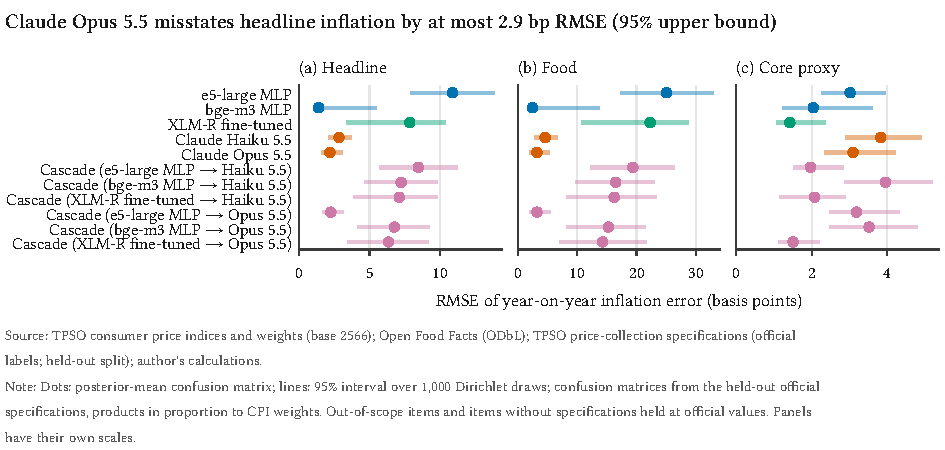
\includegraphics[width=\textwidth]{fig10_bp_error.pdf}
\caption{\textbf{\NameOpus{} misstates headline year-on-year inflation by at most
\BpYoyRmseHeadlineOpusHi{} basis points (RMSE, upper end of the \CfgCI\% interval); every
cheap method's upper end is higher.} RMSE of the year-on-year inflation error over
\NMonthsYoy{} months, headline, food and the core proxy. Dots: posterior-mean confusion matrix;
lines: \CfgCI\% interval over \CfgDraws{} Dirichlet draws. Products in proportion to CPI
weights; out-of-scope items and items without specifications held at official values. Source:
MOC; TPSO; author's calculations.}
\label{fig:bp}
\end{figure}

The \NameBge{} MLP shows why accuracy is not enough. Its weighted accuracy equals the
\NameEfive{} MLP's (\AccWBgeMLP\% against \AccWEfiveMLP\%), but its point estimate of the
headline error is \BpYoyRmseHeadlineBgeMLP{} basis points against \BpYoyRmseHeadlineEfiveMLP.
What matters is not how much weight is misclassified but whether the two items' prices
diverged. The interval for \NameBge{} is wide (\BpYoyRmseHeadlineBgeMLPLo--\BpYoyRmseHeadlineBgeMLPHi)
and the point is at its lower end, so we would not choose a classifier on this point alone. The decomposition of Section~\ref{sec:sim} shows where the
basis points come from (Figure~\ref{fig:decomp}): for the fine-tuned XLM-R, fresh
vegetables classified as fresh fruit contribute more than any other confusion, and
confusions in opposite directions partly cancel. For \NameOpus{} the two largest contributions are
out-of-scope products classified as personal care and margarine counted under oils and fats.
The wristwatches, school bags and hair dryers sent to \textsc{oos} contribute nothing: a
product sent out of scope leaves measurement without entering another item, so in the
simulator it lowers accuracy but adds no bias.

\begin{figure}[t]
\centering
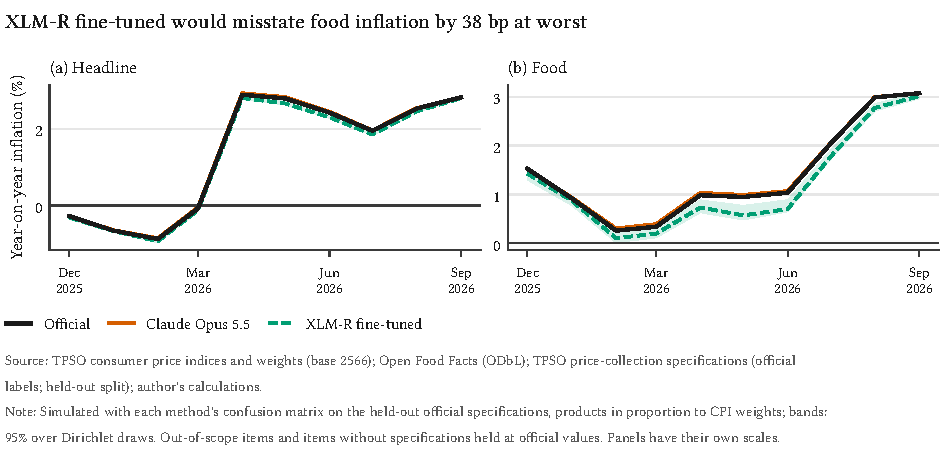
\includegraphics[width=\textwidth]{fig09_series.pdf}
\caption{\textbf{The fine-tuned XLM-R would understate food inflation in every month;
\NameOpus{} tracks the official series.} Official and simulated year-on-year inflation,
headline and food. Bands: \CfgCI\% over Dirichlet draws. Products in proportion to CPI weights.
Source: MOC; TPSO; author's calculations.}
\label{fig:series}
\end{figure}

\begin{figure}[t]
\centering
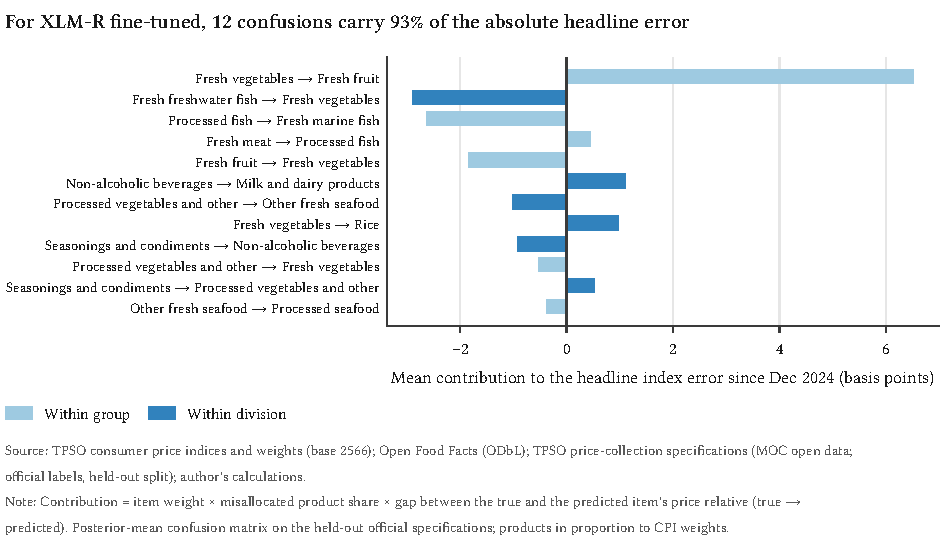
\includegraphics[width=\textwidth]{fig11_where_errors_hurt.pdf}
\caption{\textbf{A handful of confusions carry the headline error of the fine-tuned XLM-R,
and fresh vegetables classified as fresh fruit is the largest.} Mean contribution of each
confusion to the headline index error since the price reference month: item weight times
misallocated product share times the gap between the two items' price relatives. Shade: the
lowest level of the classification the two items share. Source: MOC; TPSO; author's
calculations.}
\label{fig:decomp}
\end{figure}

\paragraph{Robustness.} Three assumptions move these numbers. \emph{The product universe:} if
products arrive in proportion to the office's specification list rather than to CPI weights,
\NameOpus's headline error is \BpYoyRmseHeadlineOpusList{} basis points and the \NameEfive{}
MLP's \BpYoyRmseHeadlineEfiveMLPList. \emph{Product-level noise:} if each product's price
drifts from its item's with an annual standard deviation of \CfgSigmaHi\%, \NameOpus's
headline error rises to \BpYoyRmseHeadlineOpusNoiseTen{} basis points
[\BpYoyRmseHeadlineOpusNoiseTenLo, \BpYoyRmseHeadlineOpusNoiseTenHi], because each item is
then measured from a finite sample of products; at \CfgSigmaLo\% it is \BpYoyRmseHeadlineOpusNoiseFive.
\emph{Coverage alone:} a perfect classifier on the same universe has an error of
\BpYoyRmseHeadlinePerfect{}, so none of the error above comes from the items held at official
values.

\paragraph{Basis points need accuracy alongside.} A product sent out of scope leaves
measurement, and without product-level noise an item measured from a few correctly
classified products is measured exactly. A classifier that sends nearly everything out of
scope therefore looks good in basis points: the \NameEfive{} linear classifier trained on a
hundred official labels alone gets only \AccWEfiveLinMocHundred\% of the weight right, yet its
headline error is \BpYoyRmseHeadlineEfiveLinMocHundred{} basis points. Product-level noise
exposes it: at \CfgSigmaHi\% its error is \BpYoyRmseHeadlineEfiveLinMocHundredNoiseTen{} basis
points, against \BpYoyRmseHeadlineOpusNoiseTen{} for \NameOpus. Neither metric ranks methods
alone; a method should be chosen on both.

\section{Discussion: what this means for central banks in Asia}\label{sec:discussion}

% Written after the gold evaluation, from results only.
\textit{[This part is written once the gold labels are evaluated.]}

\section{Limitations}\label{sec:limitations}

\paragraph{One labeller.} The gold labels are the author's. The second pass measures how
consistent one person is with themselves, not how far two trained annotators would disagree,
so the label ceiling of Section~\ref{sec:results} is optimistic. Gold labels can also be
wrong in ways that favour a model which shares the labeller's reading of the item headings.

\paragraph{The product universe is Open Food Facts.} The gold frame is the Thai-script
products in a crowd-sourced database, not the assortment of Thai shops. It over-represents
packaged, branded products that volunteers chose to enter, and the universe shares $n_k$ in
the simulator are shares of that frame. A statistical office would draw the frame from its
own scanner or web data, where the mix of items, and therefore the error in basis points,
may differ.

\paragraph{Item weights below the published cells are estimated.} TPSO publishes weights for
its aggregates only. The equal split and the NNLS split are two transparent estimates; they
agree on the cells but not on the items inside them. Results that depend on which item
inside a cell carries the weight are reported under both.

\paragraph{The simulator measures classification error only.} It takes official item
relatives as the true price movements of every product and changes nothing but the
assignment of products to items. A real web-price index would add sampling, matching,
quality-adjustment and outlier error on top. Three modelling
choices are assumptions rather than estimates: leaked out-of-scope products move with the
official non-food index, an item that receives no products takes its group's measured
movement, and the product-level dispersion of the noise variants is assumed, not
measured.

\paragraph{Official specifications are not shop listings.} The official labels come from
TPSO's price-collection specifications. They are short and regular;
shop and database texts are longer and noisier. The learning curve therefore
measures the value of this kind of official label, not of labelled shop data.

\paragraph{Closed models change.} The LLMs are reached through a commercial API. Model
revisions, prices and refusal behaviour can change after the run date; every response is
cached so that the numbers here can be reproduced, but not necessarily re-obtained. The
official specifications are public and may have been seen in pre-training. Local compute
is costed at an assumed price per GPU-hour.

\paragraph{Not comparable to Spectrum.} Spectrum classifies euro-area web data into the
ECOICOP 2018 subclasses \citep{bis2026spectrum}. Our taxonomy, language, product universe,
label source and metrics differ, so our numbers are not directly comparable with theirs,
and we do not compare them.

\section{Conclusion}\label{sec:conclusion}

% Written after the gold evaluation, from results only.
\textit{[This part is written once the gold labels are evaluated.]}


\bibliographystyle{plainnat}
\bibliography{refs}

\appendix
\section{Data sources and reproducibility}\label{app:repro}

\begin{table}[!htbp]
\centering\small
\caption{Data sources. Retrieval dates and SHA-256 checksums of every file are in the
repository (\texttt{data/SOURCES.md}, \texttt{data/manifest.csv}).}
\label{tab:sources}
\begin{tabularx}{\textwidth}{@{}lXl@{}}
\toprule
Source & Use & Licence \\
\midrule
Open Food Facts, Open Beauty Facts \citep{off2026} & Product text; weak labels; gold frame & ODbL \\
TPSO open API \citep{tpso2026api} & Monthly item and aggregate indices & Thai open government data \\
TPSO monthly CPI release & Price-updated weights of the aggregates & Thai government publication \\
TPSO base-year note \citep{tpso2025cpinote} & Division weights; base-year changes & Thai government publication \\
MOC open data \citep{moc2026specs} & Official specifications (official labels) & Thai open government data \\
COICOP 2018 \citep{unsd2018coicop} & Class codes of the in-scope items & Cited \\
\bottomrule
\end{tabularx}
\end{table}

The repository rebuilds every number in this paper from public sources. \texttt{make data}
downloads the sources and checks their checksums; \texttt{make models} computes the
embeddings, trains the classifiers and runs the LLMs (cached responses are replayed, so no
API call is made when the cache is present); \texttt{make eval econ agreement} scores the
methods on gold, runs the simulator and the label-ceiling analysis; \texttt{make figures
paper} draws the figures and builds this PDF. \texttt{cpilens report} writes every number
the paper prints into \texttt{paper/numbers.tex}, and a check in continuous integration
fails if the paper's sources contain a number typed by hand.
\texttt{results/run\_manifest.json} records package versions, model revisions and the
random seed (\CfgSeed).

\section{In-scope items and crosswalk}\label{app:items}

Table~\ref{tab:items} lists the in-scope items with their COICOP 2018 classes and both
estimated weights. The crosswalk from Open Food Facts category tags to these items is in
\texttt{taxonomy/off\_categories\_to\_thcpi.csv}, with the basis of each mapping (usually the TPSO item heading it follows).

\begin{table}[!htbp]
\centering\small
\caption{In-scope items. Weight: price-updated CPI weight, \% of headline, estimated inside
official weight cells by an equal split or by NNLS. Source: TPSO; UNSD; author's
calculations.}
\label{tab:items}
\begin{tabular}{@{}llp{4.4cm}rr@{}}
\toprule
Code & Item & COICOP 2018 & Equal & NNLS \\
\midrule
\inputrows{generated/items.tex}
\bottomrule
\end{tabular}
\end{table}

\section{LLM prompt}\label{app:prompt}

The system prompt opens with the instructions below. It then lists every label by CPI group
(code, Thai and English name, and what it includes) and the official examples, each as
\texttt{text -> label}. The product is sent as the user message. The full prompt is
generated by \texttt{cpilens.classify.llm.system\_prompt}.

\VerbatimInput[fontsize=\small,breaklines,frame=single]{generated/prompt.txt}

\section{Hyperparameters}\label{app:hyper}

\begin{table}[!htbp]
\centering\small
\caption{Hyperparameters, as read from the code.}
\label{tab:hyper}
\begin{tabular}{@{}ll@{}}
\toprule
Setting & Value \\
\midrule
$k$-NN: candidate $k$ & \CfgKs \\
Linear and MLP: optimiser, learning rate, weight decay & Adam, \CfgLR, \CfgWeightDecay \\
MLP: hidden units, dropout & \CfgMLPHidden, \CfgDropout \\
Batch size (at most); early-stopping patience & \CfgBatch; \CfgPatience \\
Fine-tuning: epochs (at most), batch, learning rate & \CfgFtEpochs, \CfgFtBatch, \CfgFtLR \\
Fine-tuning: maximum input length (tokens) & \CfgFtMaxLen \\
LLM: official examples per item; maximum output tokens & \CfgFewShot; \CfgMaxTokens \\
Cascade: candidate thresholds (the last routes every product) & \CfgThresholds \\
Official-label budgets & \CfgBudgets{} and all \\
Bootstrap resamples; simulator draws; prior weight $\alpha$ & \CfgBoot; \CfgDraws; \CfgAlpha \\
Noise variants: annual dispersion (\%) & \CfgSigmaLo, \CfgSigmaHi \\
Gap between labelling passes (hours, at least) & \CfgGapHours \\
\bottomrule
\end{tabular}
\end{table}

\section{Compute and cost ledger}\label{app:costs}

Every billed API call is logged with its tokens and cost in \texttt{results/llm\_costs.csv};
Table~\ref{tab:costs} sums it. Input tokens include prompt-cache writes and reads, which are
billed at different rates.

\begin{table}[!htbp]
\centering\small
\caption{LLM calls and cost (USD) by model and stage. Smoke and probe: pipeline checks;
eval: classification of the evaluation and development sets. Source: author's API logs.}
\label{tab:costs}
\begin{tabular}{@{}llrrrr@{}}
\toprule
Model & Stage & Calls & Input tokens & Output tokens & USD \\
\midrule
\inputrows{generated/costs.tex}
\bottomrule
\end{tabular}
\end{table}


\end{document}
